\documentclass{article}
\usepackage{graphicx}
\usepackage{hyperref}
\usepackage{amsmath,amssymb}

\title{\textbf{Distributed and Concurrent Programming}\\ First Assignment}

\author{
\\Matteini Mattia
\\Paganelli Alberto
}

\date{\today}

\begin{document}

\maketitle

\begin{abstract}
Il problema sottoposto è quello di creare un programma in grado di svolgere dei \textit{tasks} in maniera concorrente, massimizzando così le performance e riducendo i tempi di esecuzione.
Nello specifico si richiede di leggere ricorsivamente dei file sorgenti (.java) partendo da una determinata cartella categorizzandoli in base a quante linee hanno rispettando i parametri inseriti dall'utente (intervalli, numero massimo di linee)

\end{abstract}


\section{Architettura}
La soluzione da noi proposta è implementata in Java utilizzando un'architettura MVC, e prevede tre fasi principali:
\begin{enumerate}
    \item Lettura dei file dalla cartella (ed eventuali sotto-cartelle).
    \item Suddivisione dei file ad N agenti aventi il compito di contare le linee ed aggiornare il model.
    \item Aggiornamento a video dei file letti e degli intervalli.
\end{enumerate}

\subsection{Lettura dei file}
La lettura dei file viene eseguita in maniera massiva da un thread appositamente creato nel \textit{Controller} che processa gli eventi. Esso infatti fa partire il conteggio ogni qualvolta viene innescato l'evento dalla \textit{View}.
Sarà quindi quest'ultimo a suddividere il blocco di file ai thread lavoratori.


\subsection{Distribuzione del carico}
La suddivisione del lavoro avviene in maniera molto semplice. Si creano tanti blocchi di file quanti sono i threads a disposizione.
\\
Nel caso in cui il numero di file non sia esattamente un multiplo del numero di threads, verrà creato un blocco più grande per l’ultimo thread (scelta ottimizzabile).
\\
Siccome il conteggio delle linee, una volta letto il file, è un'operazione prettamente CPU bound, avere tanti thread quanti core permette di parallelizzare fisicamente i tasks. Abbiamo deciso quindi di utilizzare un numero di threads equivalente al numero di core fisici della macchina + 1 (che andrà a colmare gli eventuali momenti  di \textit{interleaving}). 
\\
In questa maniera la lettura dei file e la distribuzione del carico rimane sequenziale, si poteva optare per un'architettura in grado di distribuire anche la prima fase (come verrà specificato in seguito).


\subsection{Aggiornamento della grafica}
L’ultima fase prevede l’aggiornamento in interattivo della GUI. Per far sì che questa non fosse un’operazione bloccante si sono demandate le operazioni di update della grafica all’Event Dispatcher Thread, attraverso l’invocazione del metodo \textit{invokeLater} presente nelle \texttt{SwingUtilities}.


\subsection*{Alternativa Producer/Consumer}
Un altro possibile approccio adottabile sarebbe utilizzare un’architettura Producer/Consumer, la quale andrebbe ad ottimizzare anche la lettura iniziale dei file, distribuendo sin da subito il carico di lavoro. In tal caso, grazie al buffer si potrebbero eseguire in maniera concorrente le letture dei file e l’aggiornamento dei conteggi delle linee. In questo modo inoltre, iniziando subito la distribuzione, si otterrebbe un vantaggio importante in termini di tempo e maggiore scalabilità.


\section{Modellazione}

\subsection{Monitor}
Per gestire l'accesso concorrente alle strutture dati condivise tra i vari threads è stato utilizzato un monitor.
Il monitor gestisce l'accesso alle strutture dati contenenti le distribuzioni e i file più grandi, garantendo l'atomicità delle operazioni che le vanno a modificare.
Grazie al monitor si riesce a far fronte alle problematiche relative alla concorrenza più comuni come \textit{lost updates} e \textit{deadlock}.


\clearpage
\subsection{Rete di Petri}

\begin{figure}[h]
	\centering
	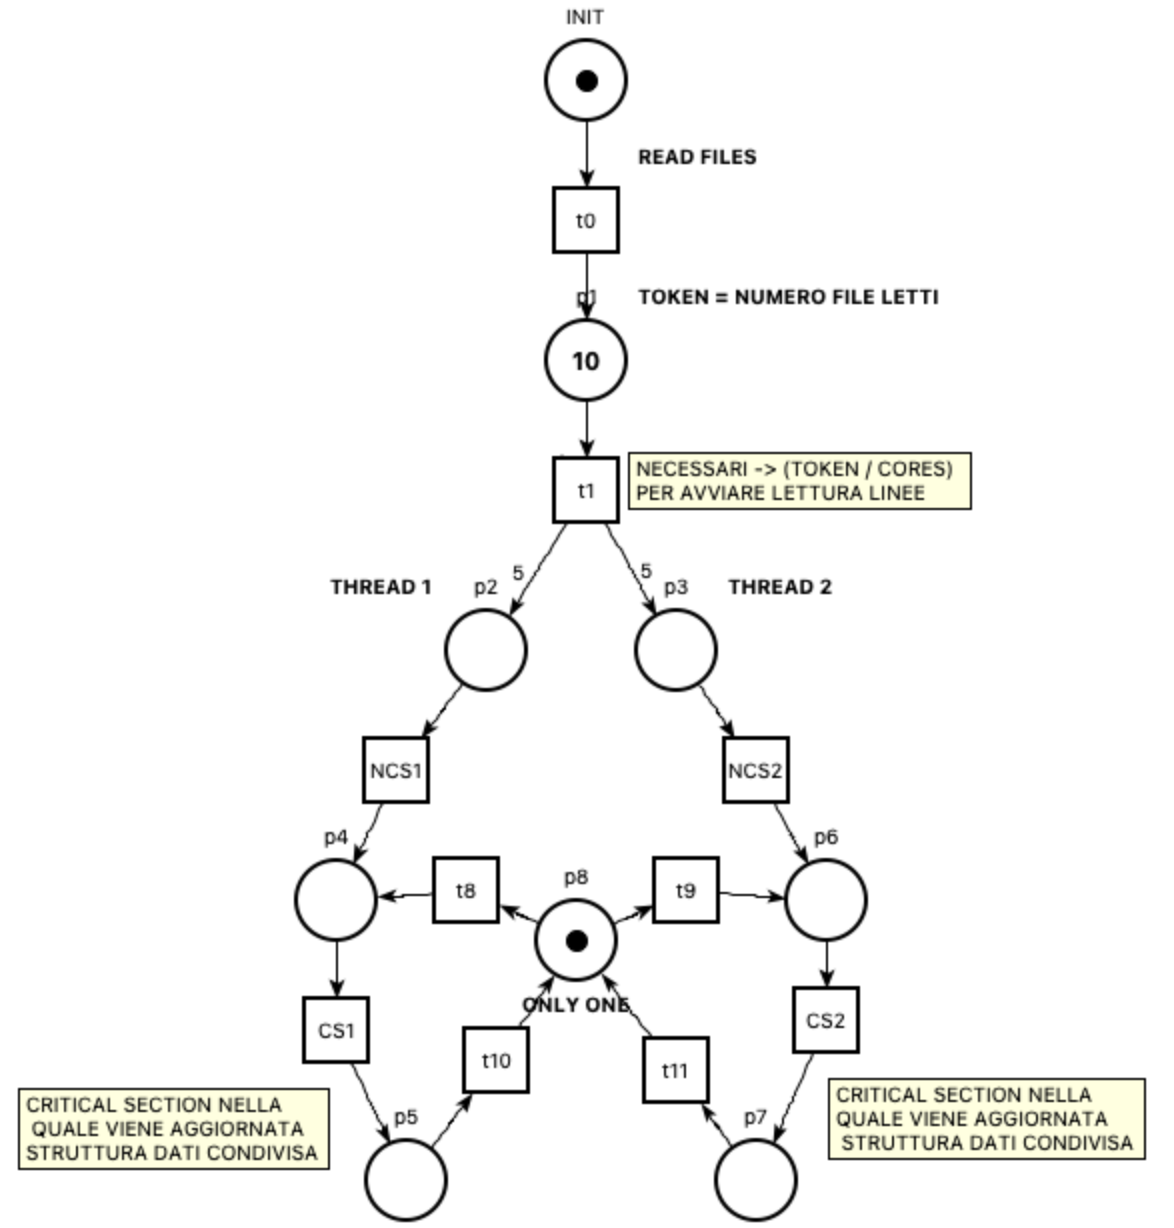
\includegraphics[width=1\linewidth]{petri-net.png}
	\caption{Rete di Petri}
	\label{fig:petri-net}
\end{figure}

\subsection{TLA+ / +CAL}
Per il modello TLA+ si è deciso di astrarre i file con delle semplici stringhe, dove i caratteri rappresentano le linee.
Sono state definite poi le seguenti proprietà temporali:

\begin{equation} \label{eq:1}
\begin{split}
    MutualExclusion == \forall i,j \mid (i \neq j) \Rightarrow \ \square\lnot (pc[i] = CS \land pc[j] = CS) \\
\end{split}
\end{equation}

\begin{equation} \label{eq:2}
    ProperFinalStringsCounter == \lozenge(counted\_strings = Len(strings))
\end{equation}

\begin{equation} \label{eq:3}
    ProperFinalCharsCounter == \lozenge(counted\_chars = \sum_{s \in strings} s.length )
\end{equation}

In (\ref{eq:1}) si verifica che due processi non entrino mai contemporaneamente in sezione critica, mentre in (\ref{eq:2}) e (\ref{eq:3}) si verifica rispettivamente che non ci siano stati \textit{lost updates}, ovvero che ``prima o poi'' i contatori raggiungano i valori corretti.


\section{Risultati Computazionali}
Il programma è stato testato selezionando in input una cartella con 2000 file sorgenti con 5000 righe di codice l'uno.
Di seguito sono mostrati i risultati dei test effettuati \footnote{I test sono stati effettuati senza l'utilizzo della cache. L'architettura utilizzata è ARM (Apple Silicon M1 Pro) con 10 core.} esprimendo in media il tempo impiegato:
\begin{itemize}
    \item 11 threads $\Rightarrow 300 ms$
    \item 8 threads $\Rightarrow 480 ms$
    \item 4 threads $\Rightarrow 700 ms$
    \item 1 threads $\Rightarrow 1250 ms$
\end{itemize}
Si nota quindi che la versione concorrente del programma quindi guadagna fino un 5x di \textit{speed up} rispetto a quella standard.

\clearpage

\section{GUI}
\begin{figure}[h]
	\centering
	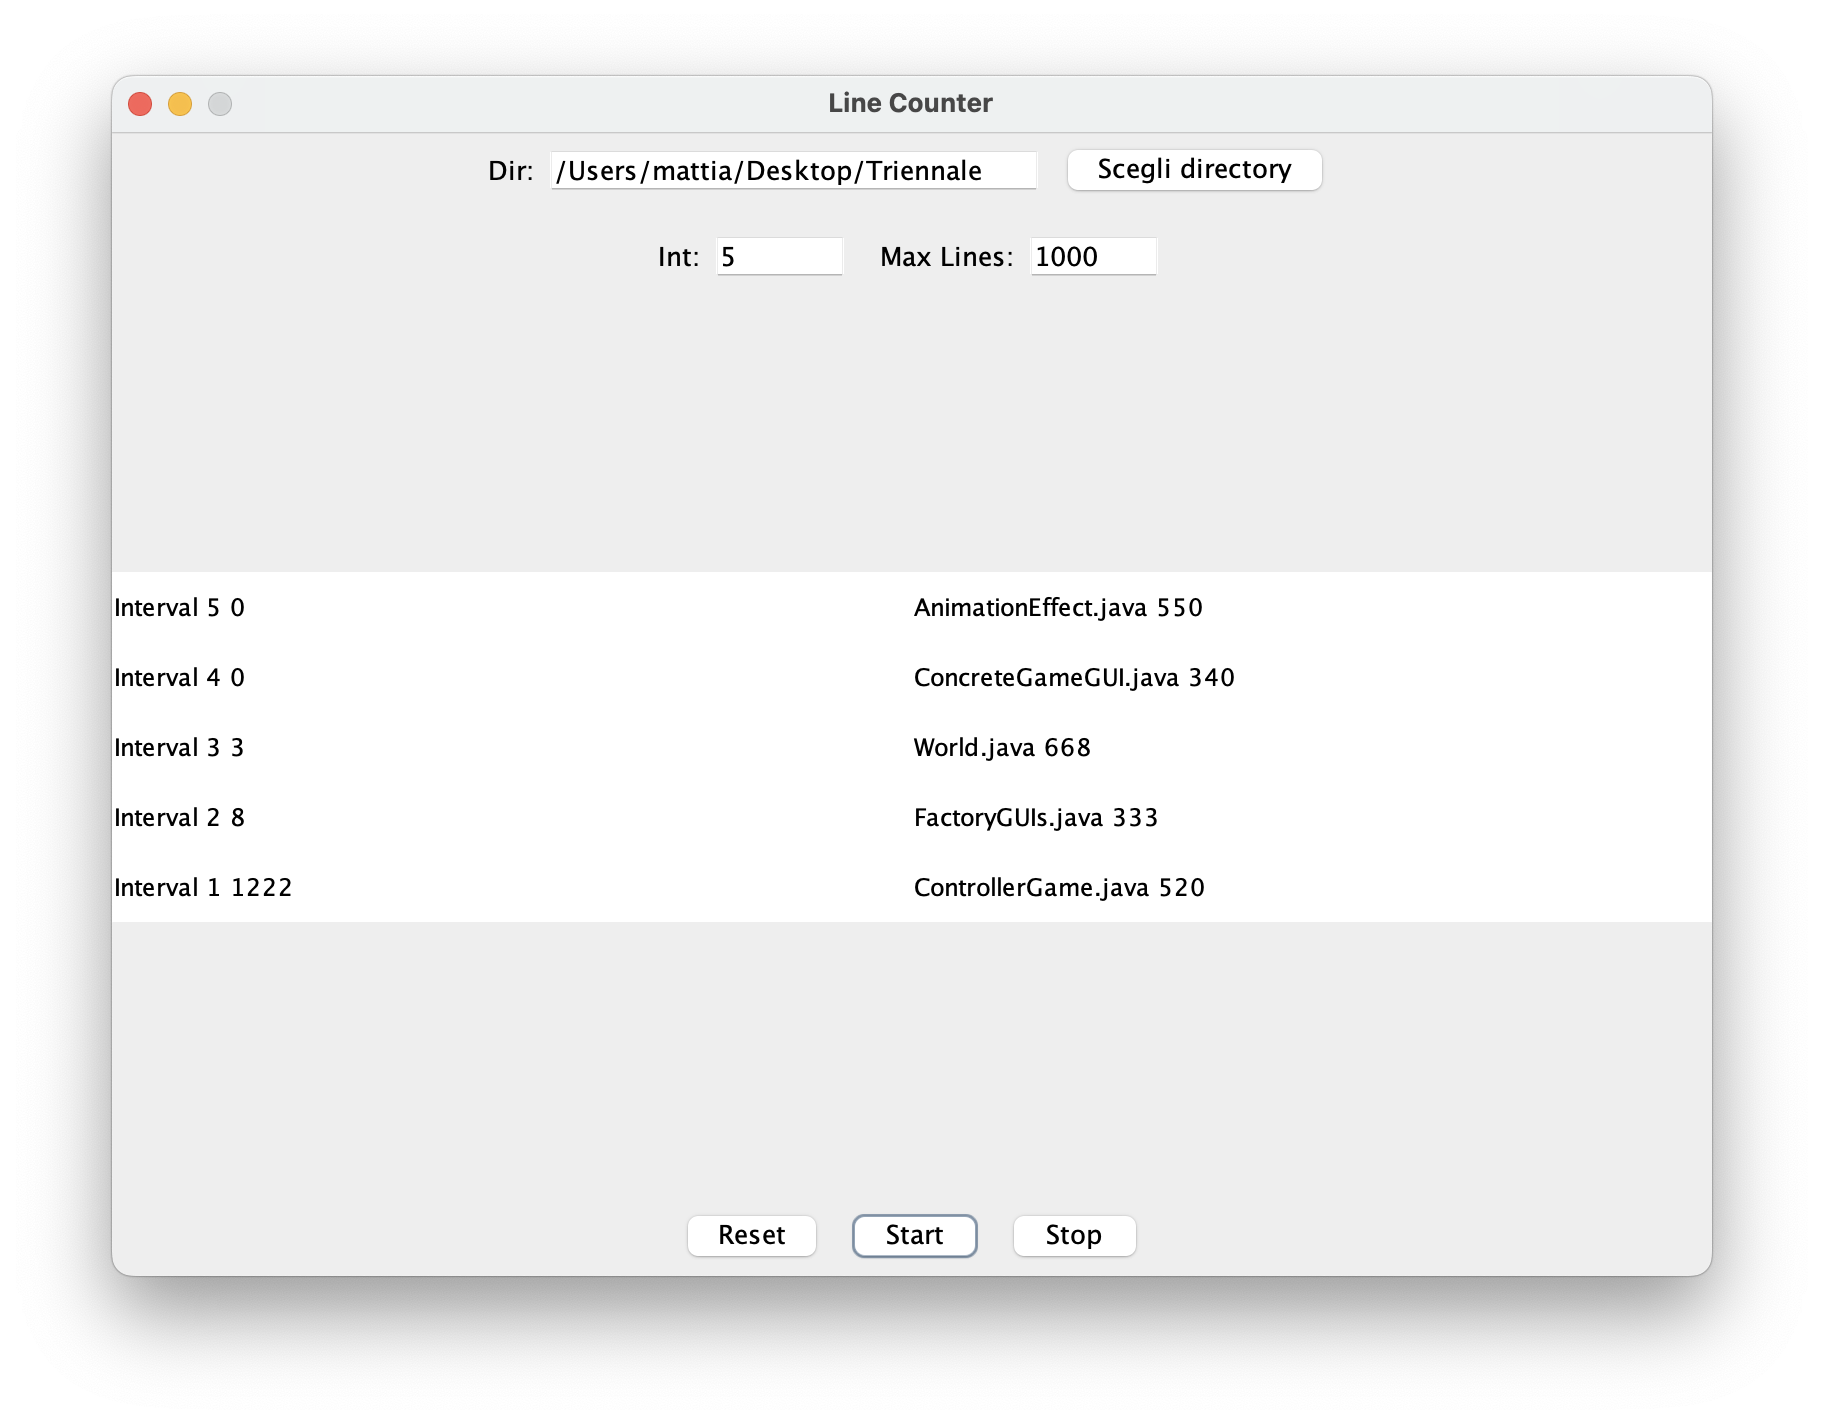
\includegraphics[width=1\linewidth]{screen-gui.png}
	\caption{Screen GUI}
	\label{fig:screen-gui}
\end{figure}

\end{document}